\documentclass[english,11pt,table,handout]{beamer}

% Copyright 2007 by Till Tantau
%
% This file may be distributed and/or modified
%
% 1. under the LaTeX Project Public License and/or
% 2. under the GNU Public License.
%
% See the file doc/licenses/LICENSE for more details.


% Common packages
\usepackage[utf8x]{inputenc}
\usepackage[vietnam,english]{babel}
\usepackage[utf8]{vietnam}
%\usepackage{times}
\usefonttheme[onlymath]{serif}
\usecolortheme{default}
\usepackage{booktabs}
\usepackage{mathpartir}
\usepackage{listings}
\usepackage{listingsutf8}

\usepackage{pbox}
\mprset{flushleft}
\mode<article>
{
  \usepackage{times}
  \usepackage{mathptmx}
  \usepackage[left=1.5cm,right=6cm,top=1.5cm,bottom=3cm]{geometry}
}

\usepackage{hyperref}
\usepackage{tikz}
\usetikzlibrary{arrows,backgrounds}
%\tikzstyle{mnode}=[circle, draw, fill=black, inner sep=0pt, minimum width=4pt]
\usepackage{colortbl}
%\usepackage{yfonts}
\usepackage{translator} % comment this, if not available


% Common settings for all lectures in this course

\def\lecturename{Image Processing and Computer Vision}

\title{\insertlecture}

\author{\textbf{LE Thanh Sach}}

\institute
{
  \textit{Faculty of Computer Science and Engineering}\\
  \textit{Ho Chi Minh University of Technology, VNU-HCM}
}

\subject{Lecturer \lecturename}

% Beamer version theme settings

\useoutertheme[height=0pt,width=2cm,right]{sidebar}
\usecolortheme{rose,sidebartab}
\useinnertheme{circles}
\usefonttheme[only large]{structurebold}

\setbeamercolor{sidebar right}{bg=black!15}
\setbeamercolor{structure}{fg=blue}
\setbeamercolor{author}{parent=structure}

\setbeamerfont{title}{series=\normalfont,size=\LARGE}
\setbeamerfont{title in sidebar}{series=\bfseries}
\setbeamerfont{author in sidebar}{series=\bfseries}
\setbeamerfont*{item}{series=}
\setbeamerfont{frametitle}{size=}
\setbeamerfont{block title}{size=\small}
\setbeamerfont{subtitle}{size=\normalsize,series=\normalfont}

\setbeamertemplate{navigation symbols}{}
\setbeamertemplate{bibliography item}[book]
\setbeamertemplate{sidebar right}
{
  {\usebeamerfont{title in sidebar}%
    \vskip1.5em%
    \hskip3pt%
    \usebeamercolor[fg]{title in sidebar}%
    \insertshorttitle[width=2cm,center,respectlinebreaks]\par%
    \vskip1.25em%
  }%
  {%
    \hskip3pt%
    \usebeamercolor[fg]{author in sidebar}%
    \usebeamerfont{author in sidebar}%
    \insertshortauthor[width=2cm,center,respectlinebreaks]\par%
    \vskip1.25em%
  }%
  \hbox to2cm{\hss\insertlogo\hss}
  \vskip1.25em%
  \insertverticalnavigation{2cm}%
  \vfill
  \hbox to 2cm{\hfill\usebeamerfont{subsection in
      sidebar}\strut\usebeamercolor[fg]{subsection in
      sidebar}\insertshortlecture.\insertframenumber\hskip5pt}%
  \vskip3pt%
}%

\setbeamertemplate{title page}
{
  \vbox{}
  \vskip1em
  {\huge Chapter \insertshortlecture\par}
  {\usebeamercolor[fg]{title}\usebeamerfont{title}\inserttitle\par}%
  \ifx\insertsubtitle\@empty%
  \else%
    \vskip0.25em%
    {\usebeamerfont{subtitle}\usebeamercolor[fg]{subtitle}\insertsubtitle\par}%
  \fi%     
  \vskip1em\par
  \emph{\lecturename}\ 
  %on \insertdate\par
  \vskip3em\par

  \leftskip=0pt plus1fill\insertauthor\par
  \insertinstitute\vskip1em
}

\logo{
\includegraphics[width=1.5cm]{hcmut.png}}



% Article version layout settings

\mode<article>

\makeatletter
\def\@listI{\leftmargin\leftmargini
  \parsep 0pt
  \topsep 5\p@   \@plus3\p@ \@minus5\p@
  \itemsep0pt}
\let\@listi=\@listI


\setbeamertemplate{frametitle}{\paragraph*{\insertframetitle\
    \ \small\insertframesubtitle}\ \par
}
\setbeamertemplate{frame end}{%
  \marginpar{\scriptsize\hbox to 1cm{\sffamily%
      \hfill\strut\insertshortlecture.\insertframenumber}\hrule height .2pt}}
\setlength{\marginparwidth}{1cm}
\setlength{\marginparsep}{4.5cm}

\def\@maketitle{\makechapter}

\def\makechapter{
  \newpage
  \null
  \vskip 2em%
  {%
    \parindent=0pt
    \raggedright
    \sffamily
    \vskip8pt
    {\fontsize{36pt}{36pt}\selectfont Chapter \insertshortlecture \par\vskip2pt}
    {\fontsize{24pt}{28pt}\selectfont \color{blue!50!black} \insertlecture\par\vskip4pt}
    {\Large\selectfont \color{blue!50!black} \insertsubtitle\par}
    \vskip10pt

    \normalsize\selectfont Print version of
    Lecturer \emph{\lecturename} of \@date\par\vskip1.5em
    %\hfill Le Thanh Sach and Luong The Nhan, Faculty of CSE, HCMC University of Technology
  }
  \par
  \vskip 1.5em%
}

\let\origstartsection=\@startsection
\def\@startsection#1#2#3#4#5#6{%
  \origstartsection{#1}{#2}{#3}{#4}{#5}{#6\normalfont\sffamily\color{blue!50!black}\selectfont}}

\makeatother

\mode
<all>




% Typesetting Listings

\usepackage{listings}
\lstset{language=Java}

\alt<presentation>
{\lstset{%
  basicstyle=\footnotesize\ttfamily,
  commentstyle=\slshape\color{green!50!black},
  keywordstyle=\bfseries\color{blue!50!black},
  identifierstyle=\color{blue},
  stringstyle=\color{orange},
  escapechar=\#,
  emphstyle=\color{red}}
}
{
  \lstset{%
    basicstyle=\ttfamily,
    keywordstyle=\bfseries,
    commentstyle=\itshape,
    escapechar=\#,
    emphstyle=\bfseries\color{red}
  }
}



% Common theorem-like environments

\theoremstyle{example}
\newtheorem{exercise}[theorem]{\translate{Exercise}}


% New useful definitions:

\newbox\mytempbox
\newdimen\mytempdimen

\newcommand\includegraphicscopyright[3][]{%
  \leavevmode\vbox{\vskip3pt\raggedright\setbox\mytempbox=\hbox{\includegraphics[#1]{#2}}%
    \mytempdimen=\wd\mytempbox\box\mytempbox\par\vskip1pt%
    \fontsize{3}{3.5}\selectfont{\color{black!25}{\vbox{\hsize=\mytempdimen#3}}}\vskip3pt%
}}

\newenvironment{colortabular}[1]{\medskip\rowcolors[]{1}{blue!20}{blue!10}\tabular{#1}\rowcolor{blue!40}}{\endtabular\medskip}

\def\equad{\leavevmode\hbox{}\quad}

\newenvironment{greencolortabular}[1]
{\medskip\rowcolors[]{1}{green!50!black!20}{green!50!black!10}%
  \tabular{#1}\rowcolor{green!50!black!40}}%
{\endtabular\medskip}
\usepackage{pgf}

\newcommand{\Rule}[2]{\genfrac{}{}{0.7pt}{}{{\setlength{\fboxrule}{0pt}\setlength{\fboxsep}{3mm}\fbox{$#1$}}}{{\setlength{\fboxrule}{0pt}\setlength{\fboxsep}{3mm}\fbox{$#2$}}}}

\newcommand{\Rulee}[3]{\genfrac{}{}{0.7pt}{}{{\setlength{\fboxrule}{0pt}\setlength{\fboxsep}{3mm}\fbox{$#1$}}}{{\setlength{\fboxrule}{0pt}\setlength{\fboxsep}{3mm}\fbox{$#2$}}}[#3]}

\usepackage{url}

\usepackage{qtree}

\usepackage{datetime}

\usepackage{amsfonts}
\usepackage{mathtools}
\usepackage{fancybox}
\usepackage[linesnumbered]{algorithm2e}
\usepackage{ragged2e}
\usepackage{accents}

\lecture[8.1]{Representation and Description}{lecture-text}

% \subtitle{Sequence Control}

\date{09 September 2015}
\newcounter{saveenumi}

\usepackage{wrapfig}
\usetikzlibrary{automata,arrows,positioning, chains, shapes.callouts, calc}

\tikzstyle{mnode}=[circle, draw, fill=black, inner sep=0pt, minimum width=4pt]
\tikzstyle{thinking} = [draw=blue, very thick]
\edef\sizetape{1cm}
\tikzstyle{tmtape}=[draw,minimum size=\sizetape]
\tikzstyle{tmhead}=[arrow box,draw,minimum size=.5cm,arrow box
arrows={east:.25cm, west:0.25cm}]
\tikzset{
  level/.style   = { ultra thick, blue },
  connect/.style = { dashed, red },
  notice/.style  = { draw, rectangle callout, callout relative pointer={#1} },
  label/.style   = { text width=4cm }
}

\begin{document}

\begin{frame}
\selectlanguage{english}
  \maketitle
\end{frame}

\begin{frame}\frametitle<presentation>{Overview}
  \tableofcontents
\end{frame}

%%%%%%%%%%%%%%%%%%%%%%%%%%%%%%%%%%%%%%%%%%%%%%%%%%%%%%%%%%%%%%%%%%%%%
%%%%%%%%%%%%%%%%%%%%%%%%%%%%%%%%%%%%%%%%%%%%%%%%%%%%%%%%%%%%%%%%%%%%%

\section{Representation}
\subsection{Boundary following}
\frame
{
	\frametitle{Representation: Boundary Following}
	\textbf{Algorithm:}
	\begin{block}{\textbf{\alert{Step 1: }} Initialization}
	\end{block}
	\begin{itemize}
		\item $b_0$: The uppermost and leftmost point belonging to the region
		\item $c_0$: The west neighbor of $b_0$
	\end{itemize}
	\begin{figure}[!h]
		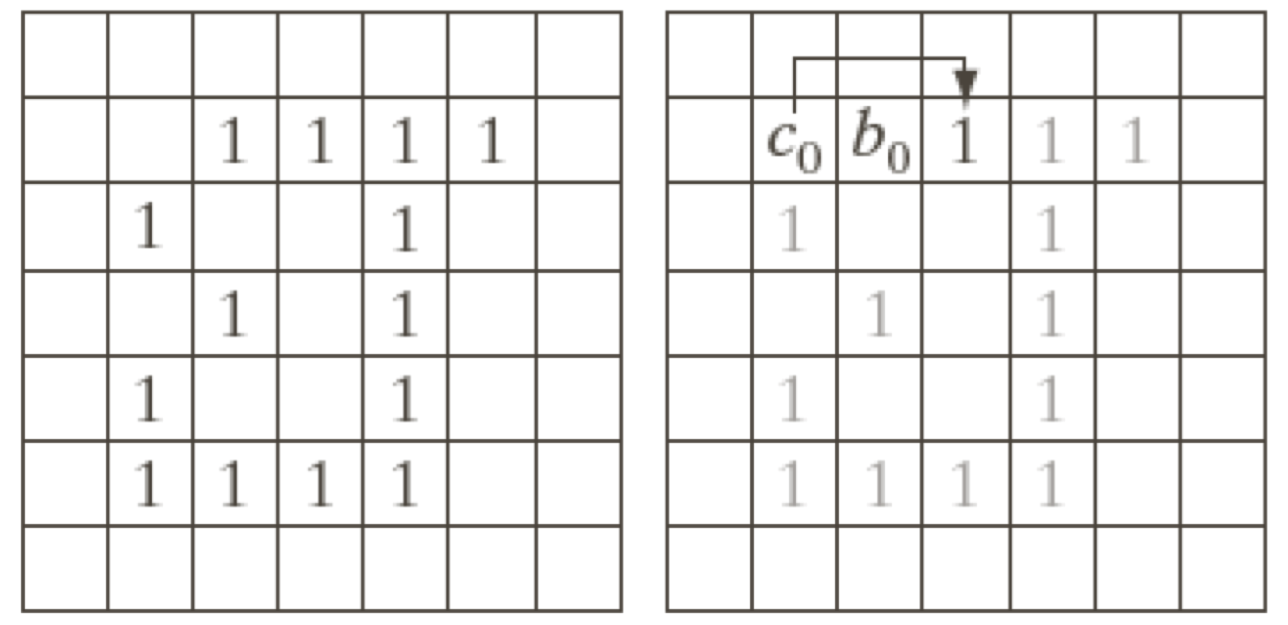
\includegraphics[width=10cm]{bfollow_1.png}
	\end{figure}
	
	
}
\frame
{
	\frametitle{Representation: Boundary Following}
	\textbf{Algorithm:}
	\begin{block}{\textbf{\alert{Step 2: }} Finding next point}
	\end{block}
	\begin{itemize}
		\item Let the 8-neighbors of $b_0$, starting at $c_0$ and proceeding in the clockwise direction be denoted as $n_1, n_2, .., n_8$
		\item Find the first $n_k$ in this sequence such that $n_k = 1$
		\item Update $b_1=n_k$ and $c_1=n_{k-1}$
	\end{itemize}
	\begin{figure}[!h]
		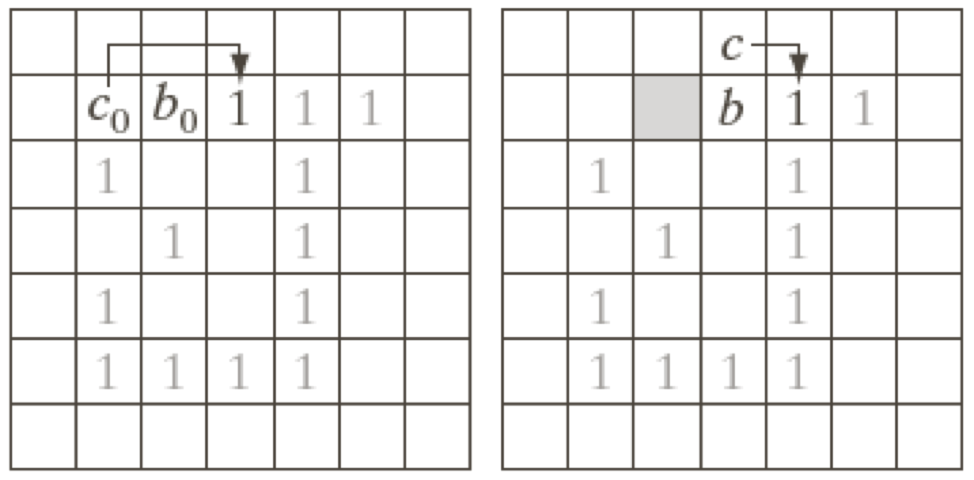
\includegraphics[height=4cm]{bfollow_2.png}
	\end{figure}	
}
\frame
{
	\frametitle{Representation: Boundary Following}
	\textbf{Algorithm:}
	\begin{block}{\textbf{\alert{Step 3: }} Finding next point}
	\end{block}
	\begin{itemize}
		\item Let $b = b_1$ and $c = c_1$
		\item Let the 8-neighbors of $b$, starting at $c$ and proceeding in the clockwise direction be denoted as $n_1, n_2, .., n_8$
		\item Find the first $n_k$ in this sequence such that $n_k = 1$
		\item Update $b=n_k$ and $c=n_{k-1}$
	\end{itemize}
	\begin{figure}[!h]
		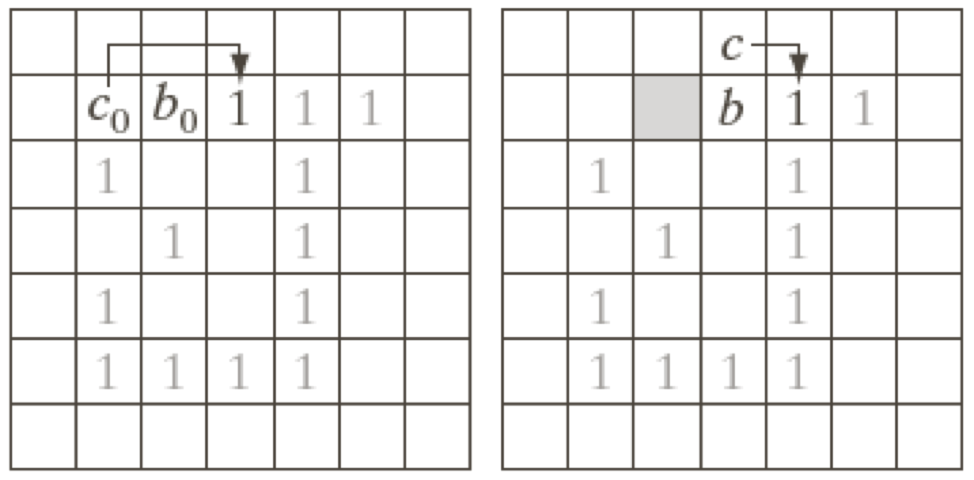
\includegraphics[height=4cm]{bfollow_2.png}
	\end{figure}	
}

\frame
{
	\frametitle{Representation: Boundary Following}
	\textbf{Algorithm:}
	\begin{block}{\textbf{\alert{Step 4: }} Iteration}
	\end{block}
	\begin{itemize}
		\item Repeat \textbf{\alert{Step 3}} until
			\begin{enumerate}
				\item $b = b_0$ \textbf{\alert{AND}} 
				\item The next boundary point of $b$ is $b_1$
			\end{enumerate}
	\end{itemize}
	\begin{figure}[!h]
		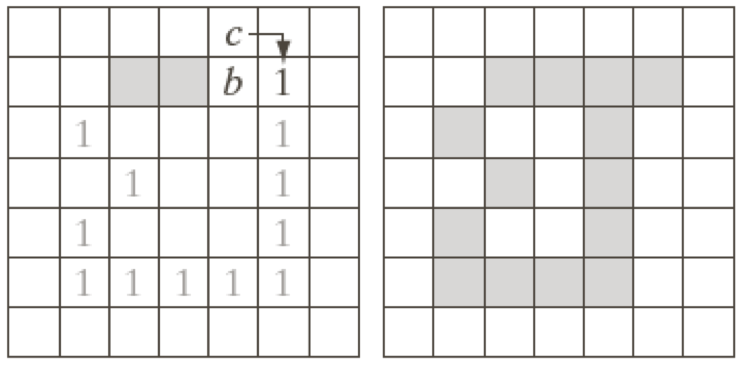
\includegraphics[height=4cm]{bfollow_3.png}
	\end{figure}	
	
}

\frame
{
	\frametitle{Representation: Boundary Following}
	\textbf{Algorithm:}
	\begin{alertblock}{Questions}
		\begin{enumerate}
			\item How does the algorithm work, if the stopping condition is only $b = b_0$, as shown in the following figure?
			\item How can we detect the boundary of holes, i.e., zero-values surrounded with 1-values.
		\end{enumerate}
	\end{alertblock}
	
	\begin{figure}[!h]
		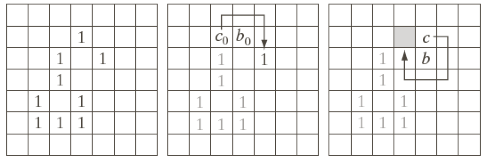
\includegraphics[width=10cm]{bfollow_4.png}
	\end{figure}	
}

\subsection{Chain codes}
\frame
{
	\frametitle{Representation: Chain codes}
	\begin{block}{Definition}
		\textbf{\alert{Feeman chain codes}} $\equiv$ \textbf{\alert{A sequence of straight-line segments}} of specified length and direction.
	\end{block}
	Each segment, as shown below,  is denoted a number according 4- or 8-connectivity:
	\begin{figure}[!h]
		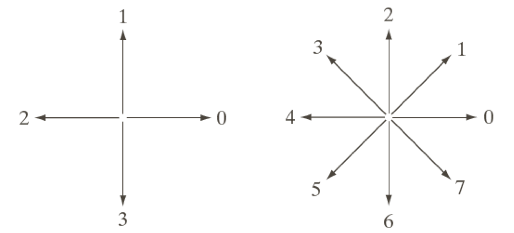
\includegraphics[width=10cm]{chaincode_1.png}
	\end{figure}
}
\frame
{
	\frametitle{Representation: Chain codes}
	\begin{block}{Algorithm for extracting chain codes}
		\begin{enumerate}
			\item Re-sample the boundary by using a larger grid spacing
			\item For each boundary point (during boundary traversing)
			\begin{enumerate}
				\item Obtain the node in the larger grid that is nearest to the current boundary point.
				\item If this node is different to the node in previous step,
				\begin{itemize}
					\item Compute a code using 4- or 8-connectivity from the node in the previous step to the current node
					\item Output this code.
				\end{itemize}
			\end{enumerate}
		
		\end{enumerate}
	\end{block}

}

\frame
{
	\frametitle{Representation: Chain codes}
	\begin{block}{A example}

	\end{block}

	\begin{figure}[!h]
		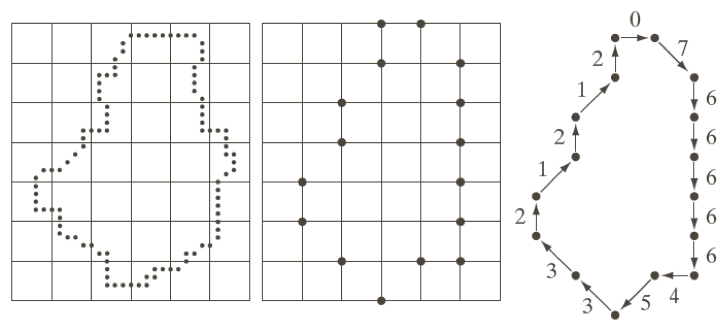
\includegraphics[width=10cm]{chaincode_2.png}
	\end{figure}
}

\frame
{
	\frametitle{Representation: Chain codes}
	\begin{alertblock}{Problems facing with chain codes}
		{
			\large
			The chain code of a boundary depends on the starting point.
		}
		
		\textbf{\textcolor{blue}{Solutions:}}
		\begin{enumerate}
			\item Sequence of codes forming the minimum integer 
			\begin{itemize}
					\item Consider the chain code as a circular sequence.
					\item Re-define the starting point so that the sequence forms an integer with minimum magnitude.
					
			\end{itemize}
			\item Sequence of differences
			 \begin{itemize}
			 	\item Difference $\equiv$ number of direction changes (e.g., in counterclockwise) between two adjacent codes.
			 \end{itemize}
		\end{enumerate}
		
	\end{alertblock}

	
}

\frame
{
	\frametitle{Representation: Chain codes}
	\begin{alertblock}{Problems facing with chain codes}
		{
			\large
			The chain code of a boundary depends on the starting point.
		}
		
		\textbf{\textcolor{blue}{Solutions:}}
		\begin{enumerate}
			\setcounter{enumi}{1}
			\item Sequence of differences
			\begin{itemize}
				\item Difference $\equiv$ number of direction changes (e.g., in counterclockwise) between two adjacent codes. For 4-connectivity:
				\begin{figure}[!h]
					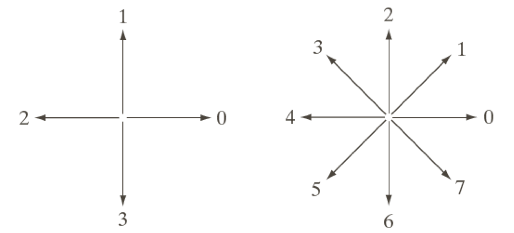
\includegraphics[width=4cm]{chaincode_1.png}
				\end{figure}
				\begin{itemize}
				\item From 1 to 0  $\equiv$ 3
				\item From 1 to 3  $\equiv$ 2
				\item From 2 to 0  $\equiv$ 2
			\end{itemize}
			\end{itemize}
			
		\end{enumerate}
		
		
	\end{alertblock}
	
}

\frame
{
	\frametitle{Representation: Chain codes}
	\begin{alertblock}{Problems facing with chain codes}
		{
			\large
			The chain code of a boundary depends on the starting point.
		}
		
		\textbf{\textcolor{blue}{Solutions:}}
		\begin{enumerate}
			\setcounter{enumi}{1}
			\item Sequence of differences
			\item Represent the chain code by a sequence of differences instead of the chain code itself.
			\item The first difference $\equiv$ the difference between the last and the first components in the original. For 4-connectivity:
			\begin{itemize}
				\item 10103322 $\rightarrow$ 33133030
			\end{itemize}
		\end{enumerate}
		
		
	\end{alertblock}
	
	
}

\frame
{
	\frametitle{Representation: Chain codes}
	\begin{figure}[!h]
		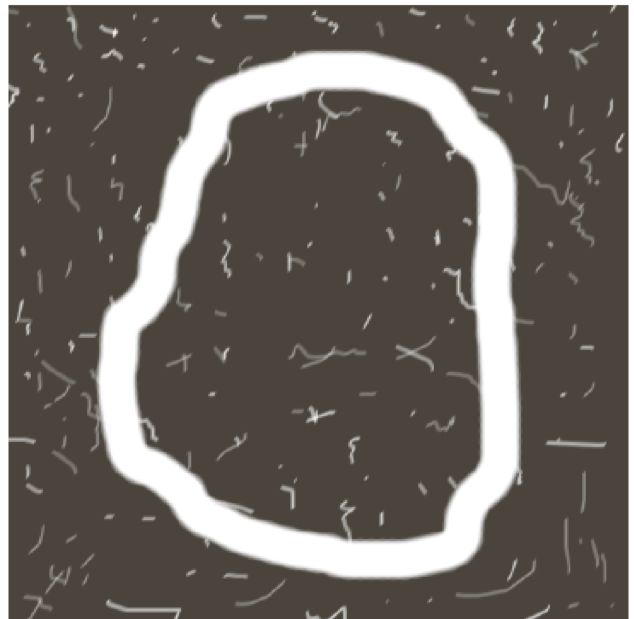
\includegraphics[height=4.5cm]{chaincode_3.png}
	\end{figure}
	
	\begin{block}{Questions}
		\begin{enumerate}
			\item How can you extract the outer and the inner boundary of the ring in the figure? Note: there are noise in the input image.
			\item How to extract the chain code that is invariant to rotation or orientation?
			
		\end{enumerate}
	\end{block}
}

\subsection{Signatures}
\frame
{
	\frametitle{Representation: Signature}
	\begin{figure}[!h]
		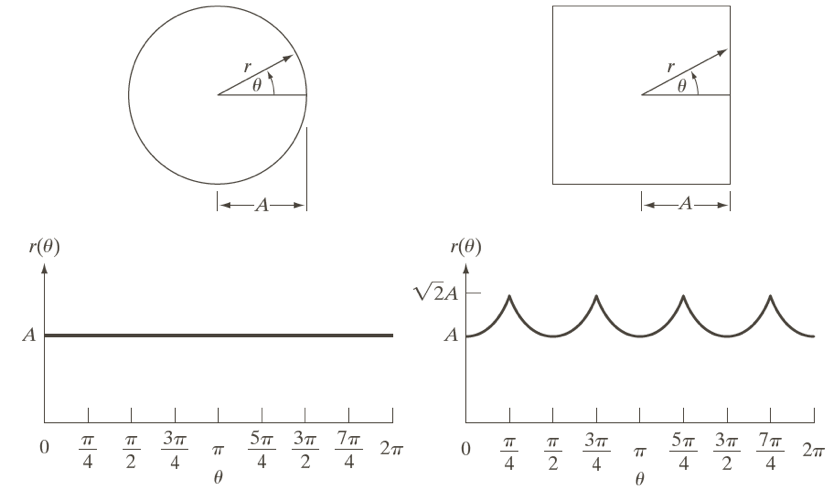
\includegraphics[height=6cm]{signature.png}
	\end{figure}
	
	\begin{alertblock}{Ideas}
		\large
		\alert{\textbf{Convert 2D boundary to 1D time series data.}}
	\end{alertblock}
}
\frame
{
	\frametitle{Representation: Signature}
	\begin{figure}[!h]
		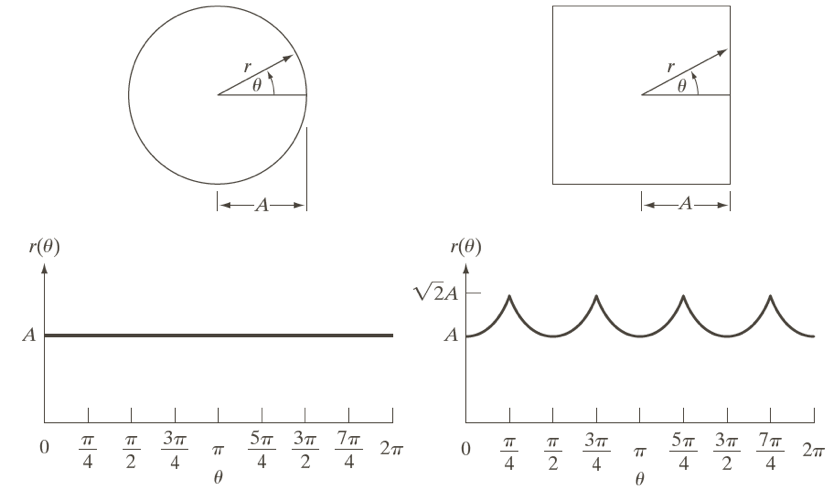
\includegraphics[height=3cm]{signature.png}
	\end{figure}
	
	\begin{block}{A Method: Distance from the centroid}
		\begin{enumerate}
			\item Determine the centroid of the boundary
			\item For each angle $\theta$ (discretized angle)
			\begin{itemize}
				\item Compute the distance from the centroid to the boundary point on the line oriented angle $\theta$ 
				\item Output this distance
			\end{itemize}
		\end{enumerate}
	\end{block}
}

\frame
{
	\frametitle{Representation: Signature}
	
	\begin{block}{Problem facing with signature}
		\begin{enumerate}
			\item Signatures depend on the starting point, not invariant to orientation (rotation)
		\end{enumerate}
		\textbf{\textcolor{blue}{Solutions:}}
		\begin{enumerate}
			\item Starting point $\equiv$ The farthest point from the centroid (assume that it is unique)
			\item Starting point $\equiv$ The farthest point on eigen-axis
		\end{enumerate}
	\end{block}
}
\frame
{
	\frametitle{Representation: Signature}
	
	\begin{block}{Problem facing with signature}
		\begin{enumerate}
			\setcounter{enumi}{1}
			\item The magnitude of signatures depends on image scaling
		\end{enumerate}
		\textbf{\textcolor{blue}{Solutions:}}
		\begin{enumerate}
			\item Normalize the magnitude to a certain range, for examples, $[0, 1]$
		\end{enumerate}
	\end{block}
}

\frame
{
	\frametitle{Representation: Signature}
	\large
	\begin{block}{Another Method: Histogram of angles}
		Input: \textbf{A reference line $L_{ref}$}
		\begin{enumerate}
			\item Extract boundary points
			\item For each point  $p$ on the boundary
			\begin{itemize}
				\item Compute tangent line $L_{tangent}$ to the boundary at $p$
				\item Compute the angle $\theta$ between $L_{tangent}$ and $L_{ref}$ 
				\item Output  $\theta$ 
			\end{itemize}
		\end{enumerate}
	\end{block}
	\begin{itemize}
		\item $L_{ref} \equiv Ox \Rightarrow$ The method 
		\item $\equiv$ Histogram of tangent angle values 
		\item $\equiv$ Slop-density function
		\item $\equiv$ Histogram of orientation for boundary points (HOG)
	\end{itemize}
}

\section{Boundary Descriptors}
\subsection{Basic Descriptors}
\frame
{
	\frametitle{Basic Boundary Descriptors}
	\large
	\begin{block}{Perimeter}
		Perimeter is the length of boundary.
		
		\textcolor{blue}{\textbf{Approximation methods:}}
		\begin{enumerate}
			\item $\equiv$ The number of pixels on the boundary.
			\item $\equiv N_e + N_o\sqrt{2}$
			\begin{itemize}
				\item $N_e$ : Number of even codes in chain code representation
				\item $N_o$ : Number of odd codes in chain code representation
			\end{itemize}
		\end{enumerate}
	\end{block}
	\begin{figure}[!h]
		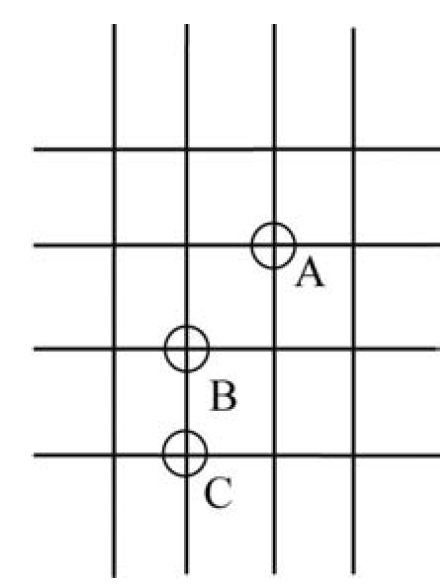
\includegraphics[height=3cm]{perimeter.png}
	\end{figure}
	\begin{itemize}
		\item distance(B,C) = 1; but, distance(A,B) = $\sqrt{2}$
	\end{itemize}
}

\frame
{
	\frametitle{Basic Boundary Descriptors}
	\large
	\begin{block}{Diameter}
		Diameter is the largest distance between any two points on a boundary.
		\vskip 2em
		\textcolor{blue}{\textbf{Mathematical Definition:}}
		\begin{itemize}
			\item $Diam(B)$: Diameter of boundary $B$
			\item $D(p_i, p_j)$: The distance between two points $p_i$ and $p_j$ on the boundary $B$
		\end{itemize} 
		\vskip 2em
		\begin{equation}
		\begin{split}
		\nonumber
		Diam(B) &= \underaccent{(i,j)}{\text{\alert{\textbf{max}}}}\{D(p_i,p_j)\}
		\end{split}
		\end{equation}
	\end{block}

}
\frame
{
	\frametitle{Basic Boundary Descriptors}
	\selectlanguage{english}
	\large
	\begin{figure}[!h]
		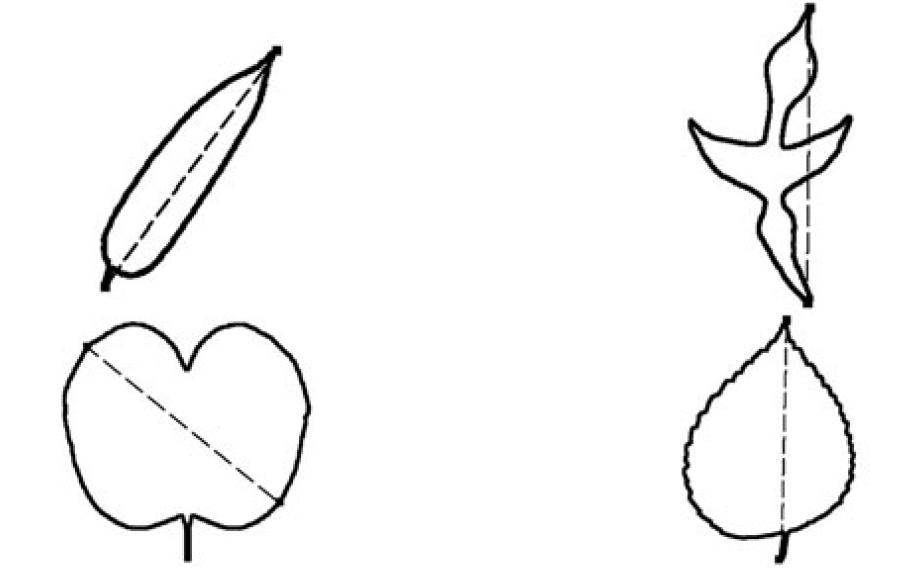
\includegraphics[width=8cm]{diameter.png}
		\caption{Diameter demonstration (Source: Book on Shape Classification and Analysis)}
	\end{figure}
}

\frame
{
	\frametitle{Basic Boundary Descriptors}
	\selectlanguage{english}
	\large
	\begin{block}{Major and Minor Axes}
		\begin{itemize}
			\item \alert{\textbf{Major Axis}} : The direction along which the shape points are more dispersed. The distance between two farthest points on the major axis is the \textbf{diameter}.
			\vskip 2em
			\item \alert{\textbf{Minor Axis}} : The direction that is perpendicular to the major axis
		\end{itemize}
	\end{block}
}

\frame
{
	\frametitle{Basic Boundary Descriptors}
	\selectlanguage{english}
	\large
	\begin{figure}[!h]
		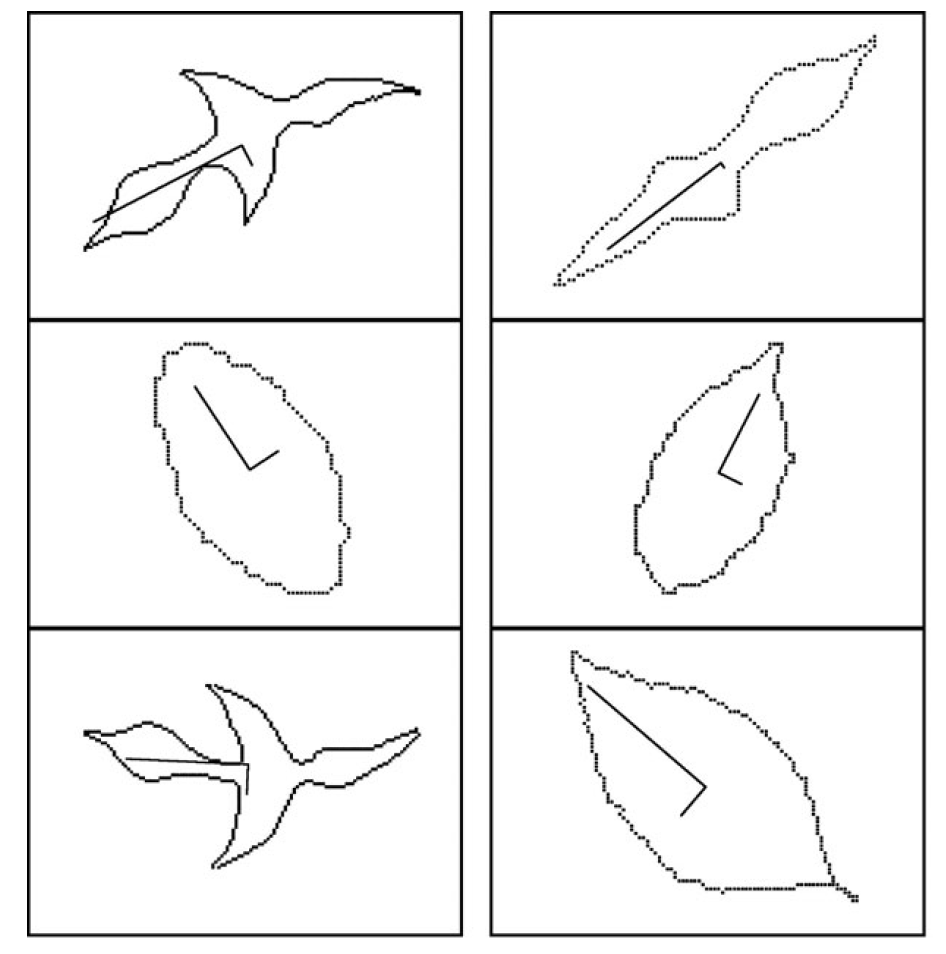
\includegraphics[width=7cm]{major_minor_axes.png}
		\caption{Demonstration of Major and Minor axes (Source: Book on Shape Classification and Analysis)}
	\end{figure}
}

\frame
{
	\frametitle{Basic Boundary Descriptors}
	\selectlanguage{english}
	\large
	\begin{block}{Algorithm for obtaining major and minor axes}
		\begin{enumerate}
			\item Extract boundary points, using boundary following algorithm. Assume that there are $n$ boundary points
			\item Store $n$ boundary points into matrix $X$ of size $n \times 2$
			\begin{itemize}
				\item Each boundary point $p(x_p, y_p)$ is stored into a row in $X$
			\end{itemize}
			\item Compute covariance matrix $K$ of $X$.
			\item Calculate the eigenvectors and eigenvalues of $K$
			\vskip 2em
			\begin{itemize}
				\item Major axis is the eigenvector corresponding to the largest eigenvalue.
				\item Minor axis is the remaining eigenvector.
			\end{itemize}
		\end{enumerate}
	\end{block}
}
\frame
{
	\frametitle{Basic Boundary Descriptors}
	\selectlanguage{english}
	\large
	\begin{block}{Basic rectangle and Eccentricity}
		\begin{itemize}
			\item \alert{\textbf{Basic rectangle}} : The rectangle is a smallest rectangle that is aligned with the major and the minor axes and completely encloses the boundary
			
			\item \alert{\textbf{Eccentricity}} : 
			\begin{equation}
				\begin{split}
					\nonumber
					E = \frac{\text{length(major axis)}}{\text{length(minor axis)}}
				\end{split}
			\end{equation}
		\end{itemize}
	
	\end{block}
}

\frame
{
	\frametitle{Basic Boundary Descriptors}
	\selectlanguage{english}
	\large
	\begin{block}{Shape number}
		\begin{itemize}
			\item \alert{\textbf{Shape number}} : The first difference (see chain-code) of smallest magnitude
			
			\vskip 2em
			\item \alert{\textbf{Order of shape}} :The order of shape $\equiv$ The number of digits in the shape number
		
		\end{itemize}
		
	\end{block}
}

\frame
{
	\frametitle{Basic Boundary Descriptors}
	\selectlanguage{english}
	
	\begin{figure}[!h]
		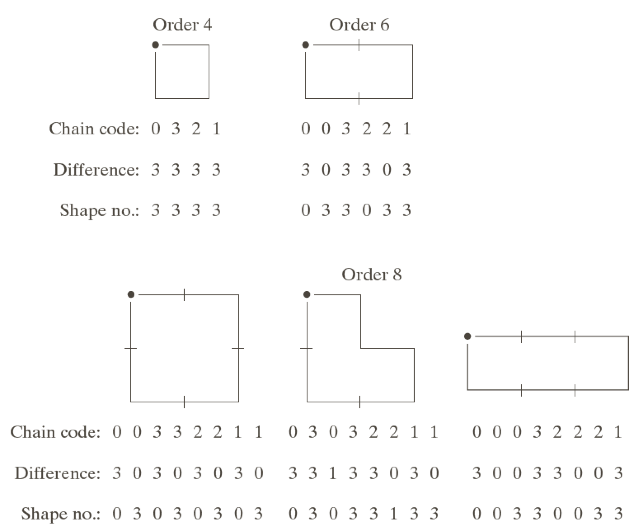
\includegraphics[width=9cm]{shape_number.png}
	\end{figure}
	Dot is the starting point
}

\frame
{
	\frametitle{Basic Boundary Descriptors}
	\selectlanguage{english}
	\begin{block}{Questions}
		Given a order, How do we obtain encode a shape in this order?
	\end{block}
	\begin{block}{Solutions}
		\begin{enumerate}
			\item Determine the basic rectangle of the shape.
			\item Calculate the eccentricity of the basic rectangle, called $E_1$
			\item From the input order, find a rectangle, called $R$, that has the order and best approximates $E_1$. 
			\begin{itemize}
				\item Input order $n=12$
				\item $\Rightarrow$ $n= 1 \times 12$ ($E=12$); $n= 2 \times 6$ ($E=3$); $n= 3 \times 4$ ($E=\frac{4}{3}$), etc.
			\end{itemize}
			\item Use $R$ to create the grid size.
			\item Use this grid to generate first difference and shape number. 
		\end{enumerate}
	\end{block}
}

\frame
{
	\frametitle{Basic Boundary Descriptors}
	\selectlanguage{english}
	
	\begin{figure}[!h]
		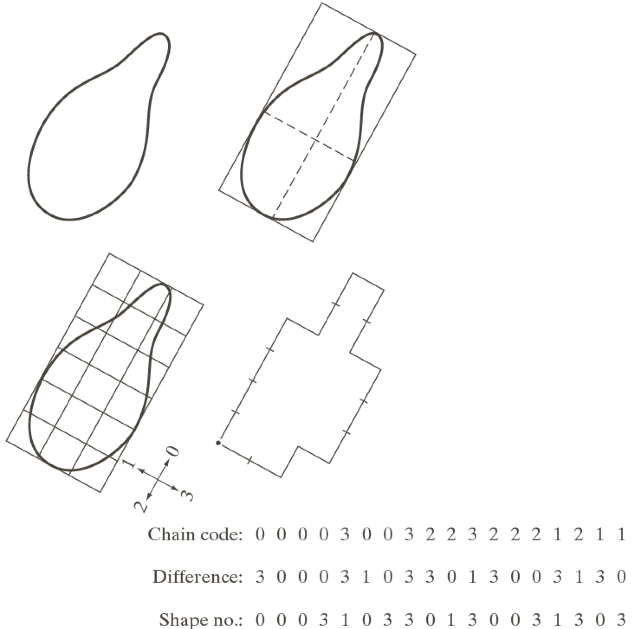
\includegraphics[width=7cm]{shape_number2.png}
		\caption{Demonstration for generating shape number from an order}
	\end{figure}
}

\subsection{Fourier Descriptors}
\frame
{
	\frametitle{Fourier Descriptors}
	\selectlanguage{english}
	\begin{block}{Input}
		\begin{itemize}
			\item A shape
		\end{itemize}
	\end{block}
	
	\begin{block}{Method}
		\begin{enumerate}
			\item Extract boundary points: $(x_0, y_0), (x_1, y_1)$, etc
			\item Define a sequence of complex numbers:
			\begin{equation}
				\begin{split}
					\nonumber
					s(k) &= x(k) + jy(k)
				\end{split}
			\end{equation}
			\begin{itemize}
				\item $x(k) = x_k; y(k) = y_k$
				\item $k = 0, 1, .., N-1$
				
			\end{itemize}
		\end{enumerate}
	\end{block}
}

\frame
{
	\frametitle{Fourier Descriptors}
	\selectlanguage{english}

	\begin{block}{Method}
		\begin{enumerate}
			\setcounter{enumi}{2}
			\item Perform Discrete Fourier Transform (DFT)
			\begin{equation}
				\begin{split}
				\nonumber
					a(u) &= \sum_{k=0}^{N-1}{s(k)e^{-j2\pi uk/N}}
				\end{split}
			\end{equation}
			\begin{itemize}
				\item $u = 0, 1, .., N-1$
				\item {\large $a(u)$ are \textbf{Fourier Descriptors}}
			\end{itemize}
			
		\end{enumerate}
	\end{block}
	
	\begin{block}{Inverse DFT}
		$s(k)$ can be approximated from the first $P$ Fourier Descriptors as follows:
		\begin{equation}
		\begin{split}
		\nonumber
			\hat{s}(k)&= \frac{1}{P} \sum_{u=0}^{P-1}{a(u)e^{j2\pi uk/N}}
		\end{split}
		\end{equation}
	\end{block}
}

\frame
{
	\frametitle{Fourier Descriptors: Example}
	\selectlanguage{english}
	
	\begin{figure}[!h]
		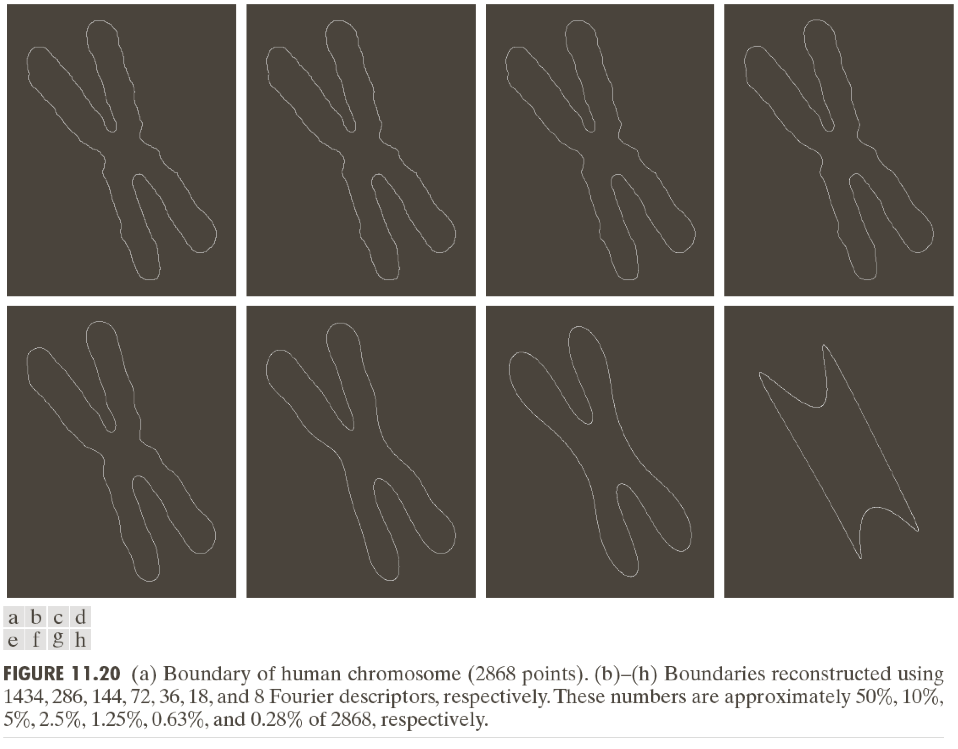
\includegraphics[width=10cm]{fourier.png}
	\end{figure}
}

\frame
{
	\frametitle{Fourier Descriptors}
	\selectlanguage{english}
	
	\begin{figure}[!h]
		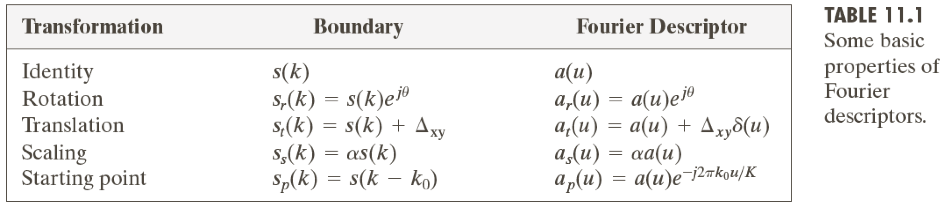
\includegraphics[width=10cm]{fourier2.png}
	\end{figure}
}
\section{Regional Descriptors}
\subsection{Simple Descriptors}
\frame
{
	\frametitle{Regional Simple Descriptors}
	\selectlanguage{english}
	\large
	\begin{itemize}
		\item \textbf{Perimeter}: defined in previous section
		\item \textbf{Area}: The number of pixels in the shape
		\item \textbf{Compactness}: 
		\begin{equation}
			\begin{split}
			\nonumber
			 \text{\textbf{Compactness}} = \frac{\text{\textbf{Perimeter}}^2}{\text{\textbf{Area}}}
			\end{split}
		\end{equation}
		\item \textbf{Circularity Ratio}: The ratio of the area of the input region to the area of the circle that has the same perimeter with the input region
		\begin{equation}
		\begin{split}
		\nonumber
			R_c = \frac{4 \pi A}{P^2}
		\end{split}
		\end{equation}
		\begin{itemize}
			\item $A$: Area of the region.
			\item $P$: Perimeter of the region.
			\item $R_c = 1 \Rightarrow$ Circle;  $R_c = \pi/4 \Rightarrow$ Square;  
		\end{itemize}
	\end{itemize}
	
}

\subsection{Topological Descriptors}
\frame
{
	\frametitle{Topological Descriptors}
	\selectlanguage{english}
	\large
	\begin{itemize}
		\item \textbf{Input}: A region has $H$ holes and $C$ connected components
		\item \textbf{Euler number}: $E = C - H$
	\end{itemize}
	
	
	\begin{figure}[!h]
		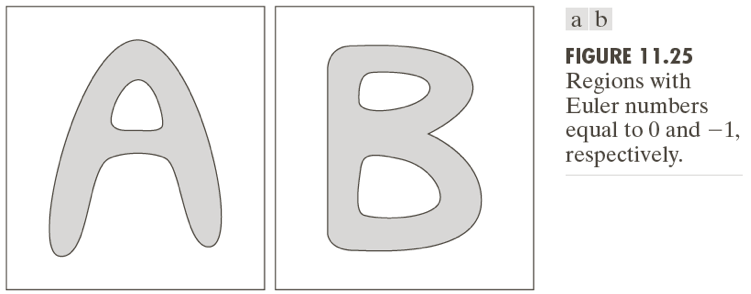
\includegraphics[width=10cm]{euler_number.png}
	\end{figure}
}

\frame
{
	\frametitle{Topological Descriptors}
	\selectlanguage{english}
	\large
	\begin{itemize}
		\item \textbf{Input}: A Region represented by straight-line segments
			\begin{enumerate}
				\item $F$ : Number of faces
				\item $V$ : Number of vertices
				\item $Q$ : Number of edges
			\end{enumerate}
		\item \textbf{Euler number}: 
	\end{itemize}
	\begin{equation}
		\begin{split}
		\nonumber
			E  &= C - H \\
			   &= V - Q + F
		\end{split}
	\end{equation}
	
	\begin{figure}[!h]
		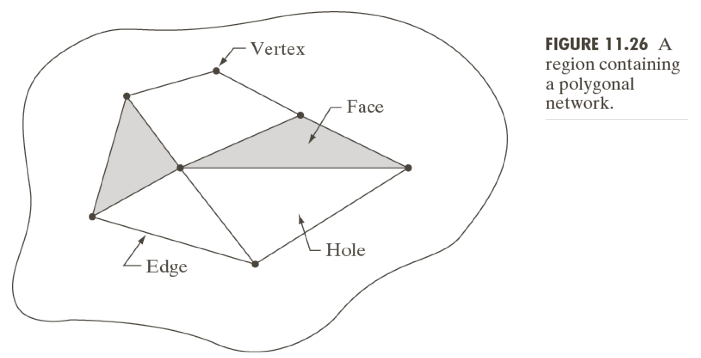
\includegraphics[width=8cm]{euler_number2.png}
	\end{figure}
}

\subsection{Texture}
\frame
{
	\frametitle{Texture: Statistical Approaches}
	\selectlanguage{english}
	\large
	\textbf{Histogram-based descriptors: }
	\newline
	
	\textbf{Input: }
	\begin{itemize}
		\item An image or a region
	\end{itemize}
	
	\begin{block}{A Method}
		\begin{enumerate}
			\item Compute histogram $p(z) = \left[p(z_0), p(z_1), p(z_i).., p(z_{L-1}) \right]$
				\begin{itemize}
					\item $i = 0, 1, ..., L-1$ ( $L=256$ for gray image)
				\end{itemize}
			\item Compute the mean of $z$
				\begin{equation}
				\begin{split}
				\nonumber
					m &= \sum_{i=0}^{L-1}{z_ip(z_i)}
				\end{split}
				\end{equation}
		\end{enumerate}
	\end{block}
	
}

\frame
{
	\frametitle{Texture: Statistical Approaches}
	\selectlanguage{english}
	\large
	\textbf{Histogram-based descriptors: }
	\newline

	\begin{block}{A Method}
		\begin{enumerate}
			\setcounter{enumi}{2}
	
			\item Compute the nth moments about the mean $m$
			\begin{equation}
			\begin{split}
			\nonumber
			\mu_n &= \sum_{i=0}^{L-1}{(z_i - m)^np(z_i)}
			\end{split}
			\end{equation}
		\end{enumerate}
	\end{block}
	
}

\frame
{
	\frametitle{Texture: Statistical Approaches}
	\selectlanguage{english}
	\large
	\textbf{Histogram-based descriptors: }
	\newline
	
	\begin{block}{Moments' meaning and properties}
		\begin{enumerate}
			\item $n=0$: $\mu_0 = 1$
			\item $n=1$: $\mu_1 = 0$
			\item $n=2$: $\mu_2 = \sigma^2$ : measure the variance of $z$ (intensities)
			\item \textbf{Relative Smoothness} $R$ is defined as
			\begin{equation}
				\begin{split}
				\nonumber
				R &= 1 - \frac{1}{1 + \sigma^2}
				\end{split}
			\end{equation}
			\begin{itemize}
				\item $R = 0$: for region of  constant intensity
				\item $R \rightarrow 1$ (approaching 1) for large variance $\sigma^2$
				\item $\sigma^2$ should be normalized to 1 by $\sigma^2 \leftarrow \sigma^2/(L-1)^2$
			\end{itemize}
		\end{enumerate}
	\end{block}
	
}
\frame
{
	\frametitle{Texture: Statistical Approaches}
	\selectlanguage{english}
	\large
	\textbf{Histogram-based descriptors: }
	\newline
	
	\begin{block}{Moments' meaning and properties}
		\begin{enumerate}
			\setcounter{enumi}{4}
			\item $n=3$: $\mu_3$ measures the skewness of the region's histogram.
			\item $n=4$: $\mu_4$ measures the flatness of the region's histogram.
			\item $n\ge 5$: still provide further \textbf{discriminative} information of texture content.
			
		\end{enumerate}
	\end{block}
	
}
\frame
{
	\frametitle{Texture: Statistical Approaches}
	\selectlanguage{english}
	\large
	\textbf{Histogram-based descriptors: }
	\newline
	
	\begin{block}{More descriptors using histogram }
		\textbf{Uniformity} $U$:
			\begin{equation}
				\begin{split}
				\nonumber
				U = \sum_{i=0}^{L-1}{p(z_i)^2}
				\end{split}
			\end{equation}
			\begin{itemize}
				\item $U$ is maximum for images in which all intensities are equal. 
			\end{itemize}
	
	\end{block}
	
}

\frame
{
	\frametitle{Texture: Statistical Approaches}
	\selectlanguage{english}
	\large
	\textbf{Histogram-based descriptors: }
	\newline
	
	\begin{block}{More descriptors using histogram }

		\textbf{Average Entropy} $E$:
		\begin{equation}
		\begin{split}
		\nonumber
		E = -\sum_{i=0}^{L-1}{p(z_i)\log_{2}{p(z_i)}}
		\end{split}
		\end{equation}
		\begin{itemize}
			\item $E$ measures the variation of intensities in images. $E = 0$ for constant images. 
		\end{itemize}
	\end{block}
	
}

\frame
{
	\frametitle{Texture: Statistical Approaches}
	\selectlanguage{english}
	\large
	\textbf{Histogram-based descriptors: }
	\newline
	
	\begin{figure}[!h]
		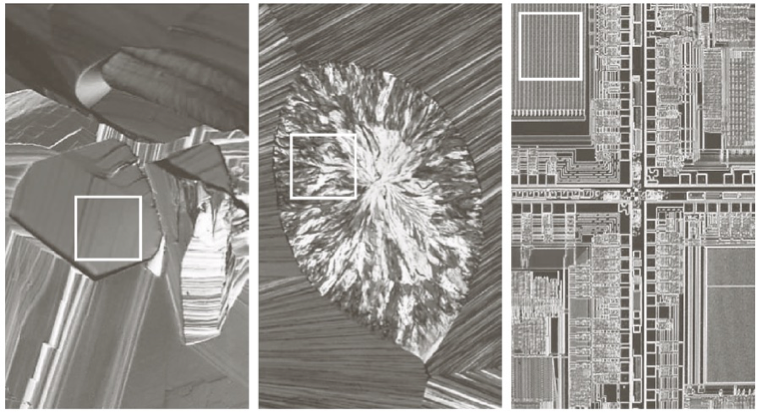
\includegraphics[width=10cm]{texture_1.png}
		\caption{Three kinds of texture in sub-images}
	\end{figure}
	
}
\frame
{
	\frametitle{Texture: Statistical Approaches}
	\selectlanguage{english}
	\large
	\textbf{Histogram-based descriptors: }
	\newline
	
	\begin{figure}[!h]
		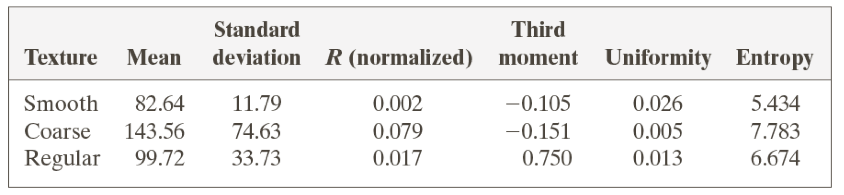
\includegraphics[width=10cm]{texture_2.png}
		\caption{Measurements for the previous three kinds of textures}. 
	\end{figure}
	Find the \textbf{discrimination} on the above measurements
	
}

\frame
{
	\frametitle{Texture: Statistical Approaches}
	\selectlanguage{english}
	\large
	\textbf{Relative positions of pixels: }
	\newline
	
	\textbf{Input:}
	\begin{itemize}
		\item An input image or a region
		\item $Q$ an operator that defines the position of two pixels relative to each other.
		\item $L$: number of intensity levels.
		\item \alert{Intensities are transformed to range of $[1, L]$ instead of $[0, L-1]$}
	\end{itemize}
	
}

\frame
{
	\frametitle{Texture: Statistical Approaches}
	\selectlanguage{english}
	\large
	\textbf{Relative positions of pixels: }
	\newline
	
	\begin{block}{Concept}
		\textbf{Co-occurrence matrix:} $G = \{g_{ij}\}_{L \times L}$
			\begin{itemize}
				\item $G$ has size of $L \times L$
				\item $i, j \in [1, L]$
			\end{itemize}
		\textbf{Meaning of} $g_{ij}$: $g_{ij}$ is the number of pairs of two pixels $p$ and $q$ that satisfy the following predicates
			\begin{itemize}
				\item $p$ and $q$ satisfy operator $Q$, for examples, they are two consecutive pixels in the input image
				\item Gray level of pixel $p$ is $i$
				\item Gray level of pixel $q$ is $j$
			\end{itemize}
		
	\end{block}
}

\frame
{
	\frametitle{Texture: Statistical Approaches}
	\selectlanguage{english}
	\large
	\textbf{Relative positions of pixels: }
	\newline
	
	\begin{examples}
		\begin{itemize}
			\item $Q$ : one pixel immediately to the right
			\item $L = 8$
			\item Input image $f$ of small size, $6 \times 6$
		\end{itemize}
		\begin{figure}[!h]
			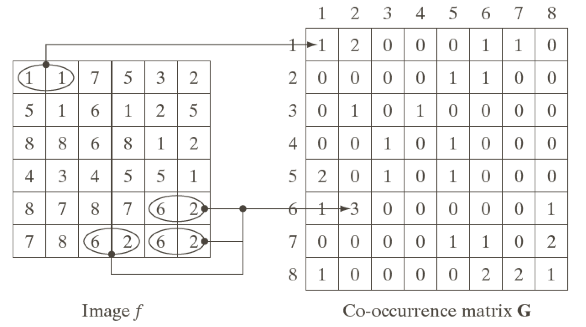
\includegraphics[width=6cm]{texture_3.png}
			\caption{Demonstration of building co-occurrence matrix }. 
		\end{figure}
	\end{examples}
}

\frame
{
	\frametitle{Texture: Statistical Approaches}
	\selectlanguage{english}
	\large
	\textbf{Relative positions of pixels: }
	\newline
	
	\begin{alertblock}{Normalized Co-occurrence Matrix: $G_{norm}$}
	
		\begin{equation}
		\begin{split}
		\nonumber
			G_{norm} = \{p_{ij} = \frac{g_{ij}}{n} \}_{L \times L}
		\end{split}
		\end{equation}
		\begin{itemize}
			\item $n$ : the total number of pairs that satisfy $Q$
		\end{itemize}
		\begin{equation}
			\begin{split}
			\nonumber
				n = \sum_{i=1}^{L}{ \sum_{j=1}^{L} {g_{ij}} }
			\end{split}
		\end{equation}
		\begin{itemize}
			\item $p_{ij}$ : probability of occurring a pair of two pixels $p$ and $q$ that satisfy the positional operator $Q$ and that they have gray-levels $i$ and $j$ respectively.
		\end{itemize}
	\end{alertblock}
}

\frame
{
	\frametitle{Texture: Statistical Approaches}
	\selectlanguage{english}
	\large
	\textbf{Relative positions of pixels: }
	\newline
	\vskip 5em
	\begin{block}{Descriptors bases on $G_{norm}$}
		\begin{enumerate}
			\item \textbf{\textcolor{blue}{Maximum Probability } }:
			\begin{equation}
			\begin{split}
			\nonumber
			 \underaccent{(i,j)}{\text{\alert{\textbf{max}}}}\{p_{ij}\}
			\end{split}
			\end{equation}
			
			\begin{itemize}
				\item Measures the strongest response of the co-occurrence
			\end{itemize}
				
		\end{enumerate}

	\end{block}
}
\frame
{
	\frametitle{Texture: Statistical Approaches}
	\selectlanguage{english}
	\large
	\textbf{Relative positions of pixels: }
	\newline
	\begin{block}{Descriptors bases on $G_{norm}$}
		\begin{enumerate}
			\setcounter{enumi}{1}
			\item \textbf{\textcolor{blue}{Correlation } }:
			
			\begin{equation}
			\begin{split}
			\nonumber
				\sum_{i=1}^{K}{ \sum_{j=1}^{K} { \frac{(i - m_r)(j - m_c)p_{ij}}{ \sigma_r \sigma_c } } }
			\end{split}
			\end{equation}
			
			\begin{itemize}
				\item Measures how correlated a pixel is to its neighbors over the entire image
				\item Range of values: $[-1, 1]$, i.e., perfect negative and perfect positive.
				\item $\sigma_r \neq 0$ and $\sigma_c \neq 0$
				
			\end{itemize}
			
		\end{enumerate}
		
	\end{block}
}

\frame
{
	\frametitle{Texture: Statistical Approaches}
	\selectlanguage{english}

	\textbf{Relative positions of pixels: }
	\newline
	\begin{block}{Descriptors bases on $G_{norm}$}
		\begin{enumerate}
			\setcounter{enumi}{1}
			\item \textbf{\textcolor{blue}{Correlation } }:
			
			\begin{equation}
			\begin{split}
			\nonumber
			m_r &= \sum_{i=1}^{K}{i \sum_{j=1}^{K}{p_{ij} } } \\
			m_c &= \sum_{j=1}^{K}{j \sum_{i=1}^{K}{p_{ij} } } \\
			\sigma_r &= \sum_{i=1}^{K}{(i - m_r)^2 \sum_{j=1}^{K}{p_{ij} } } \\
			\sigma_c &= \sum_{j=1}^{K}{(j - m_c)^2 \sum_{i=1}^{K}{p_{ij} } } 
			\end{split}
			\end{equation}
			
			
			
		\end{enumerate}
		
	\end{block}
}

\frame
{
	\frametitle{Texture: Statistical Approaches}
	\selectlanguage{english}
	\large
	\textbf{Relative positions of pixels: }
	\newline
	\begin{block}{Descriptors bases on $G_{norm}$}
		\begin{enumerate}
			\setcounter{enumi}{2}
			\item \textbf{\textcolor{blue}{Contrast } }:
			
			\begin{equation}
			\begin{split}
			\nonumber
			\sum_{i=1}^{K}{ \sum_{j=1}^{K} { (i-j)^2p_{ij} } }
			\end{split}
			\end{equation}
			
			\begin{itemize}
				\item Measures the intensity contrast between a pixel to its neighbors over the entire image.
				\item Range of values: $[0, (K-1)^2]$
				\item Contrast $= 0 \equiv$ $G$ is constant.
				
			\end{itemize}
			
		\end{enumerate}
		
	\end{block}
}

\frame
{
	\frametitle{Texture: Statistical Approaches}
	\selectlanguage{english}
	\large
	\textbf{Relative positions of pixels: }
	\newline
	\begin{block}{Descriptors bases on $G_{norm}$}
		\begin{enumerate}
			\setcounter{enumi}{3}
			\item \textbf{\textcolor{blue}{Uniformity } }:
			
			\begin{equation}
			\begin{split}
			\nonumber
			\sum_{i=1}^{K}{ \sum_{j=1}^{K} { p_{ij}^2 } }
			\end{split}
			\end{equation}
			
			\begin{itemize}
				\item Measures the uniformity
				\item Range of values: $[0, 1]$
				\item Uniformity $= 1$ for constant images
				
			\end{itemize}
			
		\end{enumerate}
		
	\end{block}
}

\frame
{
	\frametitle{Texture: Statistical Approaches}
	\selectlanguage{english}
	\large
	\textbf{Relative positions of pixels: }
	\newline
	\begin{block}{Descriptors bases on $G_{norm}$}
		\begin{enumerate}
			\setcounter{enumi}{4}
			\item \textbf{\textcolor{blue}{Homogeneity } }:
			
			\begin{equation}
			\begin{split}
			\nonumber
			\sum_{i=1}^{K}{ \sum_{j=1}^{K} { \frac{p_{ij}}{ 1 + |i - j|}  } }
			\end{split}
			\end{equation}
			
			\begin{itemize}
				\item Measures the spatial closeness of the distribution of elements in $G$ to the diagonal 
				\item Range of values: $[0, 1]$
				\item Homogeneity $= 1  \equiv $ $G$ is diagonal matrix
				
			\end{itemize}
			
		\end{enumerate}
		
	\end{block}
}

\frame
{
	\frametitle{Texture: Statistical Approaches}
	\selectlanguage{english}
	\large
	\textbf{Relative positions of pixels: }
	\newline
	\begin{block}{Descriptors bases on $G_{norm}$}
		\begin{enumerate}
			\setcounter{enumi}{5}
			\item \textbf{\textcolor{blue}{Entropy } }:
			
			\begin{equation}
			\begin{split}
			\nonumber
			\sum_{i=1}^{K}{ \sum_{j=1}^{K} { p_{ij}\log_{2}{p_{ij}} } }
			\end{split}
			\end{equation}
			
			\begin{itemize}
				\item Measures the randomness of elements in $G$ 
				\item Entropy $= 0$: all elements in $G$ are zeros
				\item Entropy $= 1$: all elements in $G$ are equal
				\item Max entropy = $2 \times \log_2{K}$
				
			\end{itemize}
			
		\end{enumerate}
		
	\end{block}
}


\frame
{
	\frametitle{Texture: Statistical Approaches - Demonstration}
	\selectlanguage{english}
	\begin{figure}[!h]
		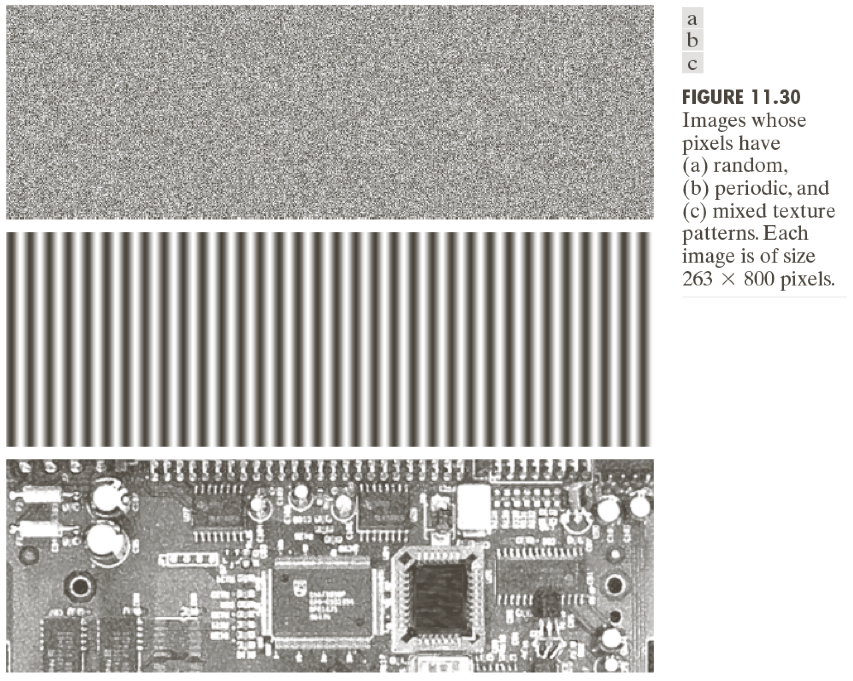
\includegraphics[width=10cm]{texture_4.png}
	\end{figure}
}

\frame
{
	\frametitle{Texture: Statistical Approaches - Demonstration}
	\selectlanguage{english}
	\begin{figure}[!h]
		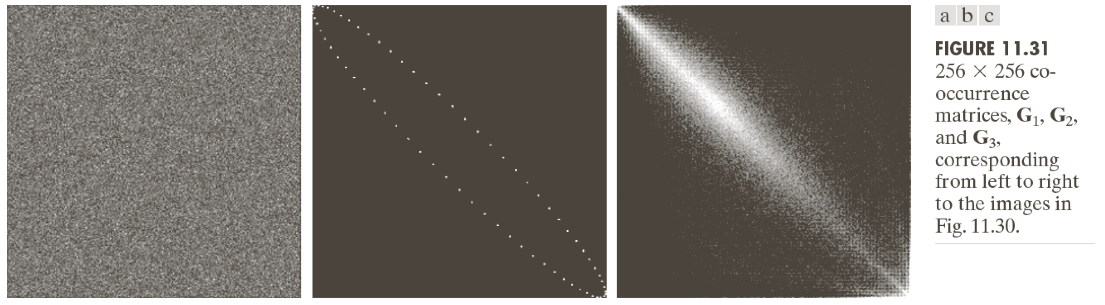
\includegraphics[width=10cm]{texture_5.png}
	\end{figure}
	\begin{itemize}
		\item $Q$: One pixel immediately to the right
		\item Note: these matrices are discriminative
	\end{itemize}
}
\frame
{
	\frametitle{Texture: Statistical Approaches - Demonstration}
	\selectlanguage{english}
	\begin{figure}[!h]
		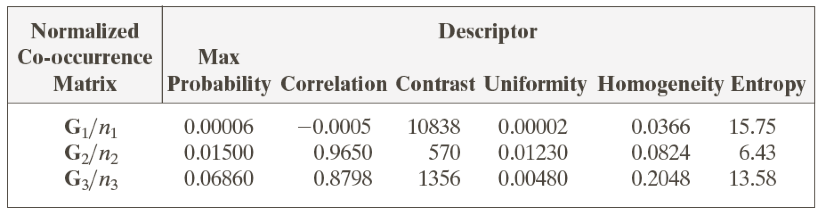
\includegraphics[width=10cm]{texture_6.png}
	\end{figure}
	\begin{itemize}
		\item Measurements are discriminative
		
	\end{itemize}
}

\frame
{
	\frametitle{Texture: Statistical Approaches}
	\selectlanguage{english}
	\begin{block}{Questions}
		How can you reduce the size of co-occurrence matrices?
		
	\end{block}
}
\subsection{Spectral Descriptors}
\frame
{
	\frametitle{Spectral Descriptors}
	\selectlanguage{english}
	\large
	\begin{block}{Method}
		\begin{enumerate}
			\item Compute FFT, called $F(u.v)$, for the input image $f(x,y)$ for sub-image containing the input region.
			\item Convert $F(u.v)$ to polar system $T(r, \theta)$
			\item Compute measurements $S(r)$ and $S(\theta)$
			
		\end{enumerate}
		\begin{equation}
		\begin{split}
		\nonumber
			S(r) &= \sum_{\theta = 0}^{\pi}{T(r, \theta) } \\
			S(\theta) &= \sum_{r = 1}^{R_0}{T(r, \theta) }
		\end{split}
		\end{equation}
		\begin{itemize}
			\item $R_0$ : the radius of a circle centered at the origin.
		\end{itemize}
	\end{block}
}

\frame
{
	\frametitle{Spectral Descriptors - Demonstration}
	\selectlanguage{english}
	\begin{figure}[!h]
		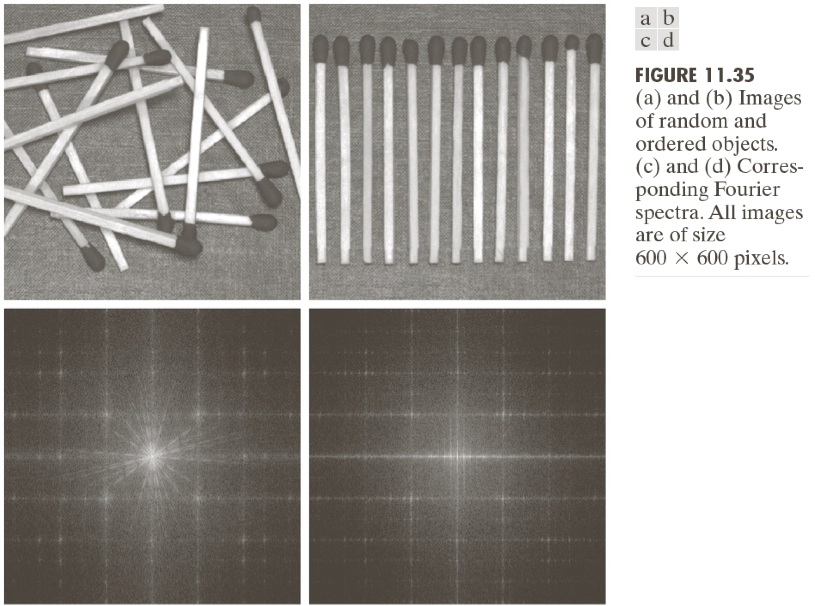
\includegraphics[width=10cm]{spectral_1.png}
	\end{figure}
}

\frame
{
	\frametitle{Spectral Descriptors - Demonstration}
	\selectlanguage{english}
	\begin{figure}[!h]
		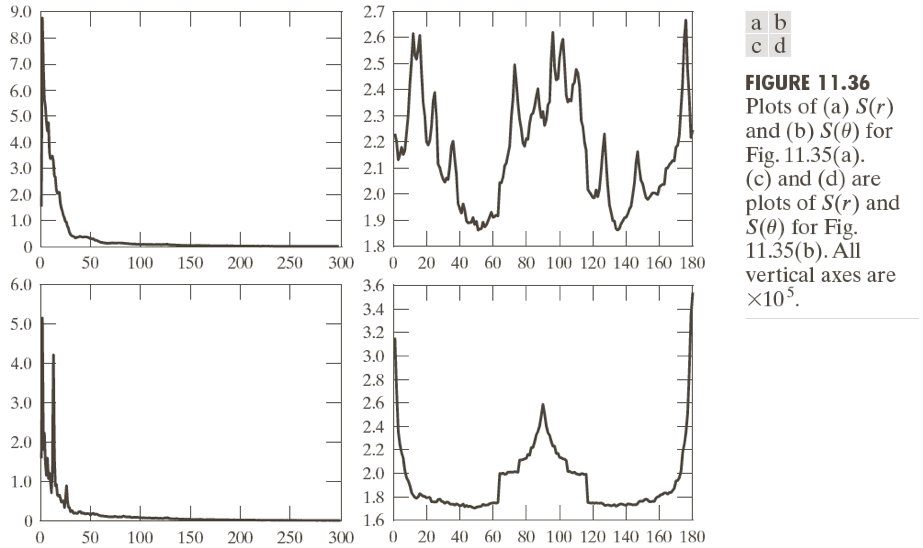
\includegraphics[width=10cm]{spectral_2.png}
	\end{figure}
}

\section{Moments}
\frame
{
	\frametitle{Moments}
	\selectlanguage{english}
	\large
	\begin{block}{Inputs}
		\begin{enumerate}
			\item Image $f(x,y)$ of size $M \times N$
		\end{enumerate}
	\end{block}
	
	\begin{alertblock}{Moments of order \textbf{(p + q) }}
		\begin{equation}
		\begin{split}
		\nonumber
			m_{pq} &= \sum_{x = 0}^{M-1}{ \sum_{y = 0}^{N-1} {x^p y^q f(x,y)} } 
		\end{split}
		\end{equation}
		\begin{itemize}
			\item $p = 0, 1, 2, ...$
			\item $q = 0, 1, 2, ...$
		\end{itemize}
	\end{alertblock}
}

\frame
{
	\frametitle{Moments}
	\selectlanguage{english}
	\large
	
	\begin{alertblock}{Central Moments of order \textbf{(p + q) }}
		\begin{equation}
		\begin{split}
		\nonumber
		\mu_{pq} &= \sum_{x = 0}^{M-1}{ \sum_{y = 0}^{N-1} {(x - \bar{x})^p (y - \bar{y})^q f(x,y)} } 
		\end{split}
		\end{equation}
		\begin{itemize}
			\item $p = 0, 1, 2, ...$
			\item $q = 0, 1, 2, ...$
		\end{itemize}
		
		\begin{equation}
		\begin{split}
		\nonumber
			\bar{x} &= \frac{m_{10} }{m_{00}} \\
			\bar{y} &= \frac{m_{01} }{m_{00}}
		\end{split}
		\end{equation}
		
	\end{alertblock}
}

\frame
{
	\frametitle{Moments}
	\selectlanguage{english}
	\large
	
	\begin{alertblock}{Set of 7 moments}
		\begin{itemize}
			\item \textcolor{blue}{See textbook on pp.863}
			\item These moments are invariant to translation, rotation, scaling and mirroring 
		\end{itemize}
		
	\end{alertblock}
}

\frame
{
	\frametitle{Moments - Demonstration}
	\selectlanguage{english}
	\begin{figure}[!h]
		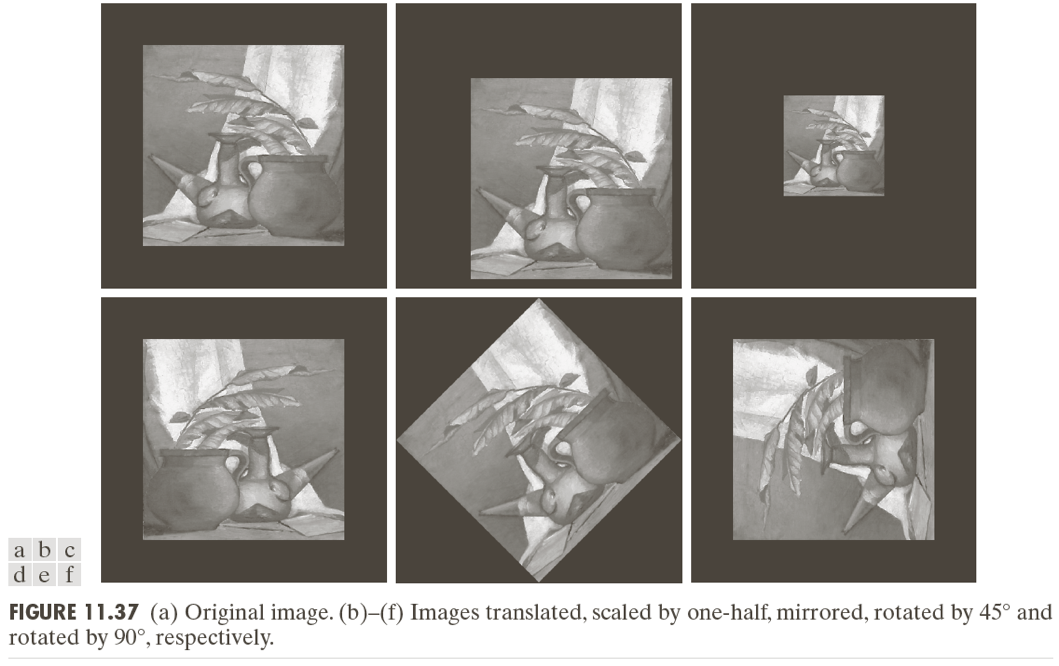
\includegraphics[width=10cm]{moment_1.png}
	\end{figure}
}

\frame
{
	\frametitle{Moments - Demonstration}
	\selectlanguage{english}
	\begin{figure}[!h]
		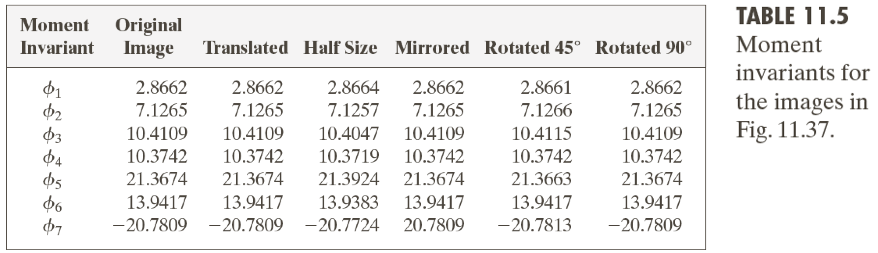
\includegraphics[width=10cm]{moment_2.png}
	\end{figure}
	\begin{itemize}
		\item Note: The value of moments just \alert{\textbf{change slightly}} with rotation, scalling, translation, and mirroring.
	\end{itemize}
}
\section{Principal Components for Description}
\subsection{Principal Components}
\frame
{
	\frametitle{Principal Components}
	\selectlanguage{english}
	\large
	\begin{block}{Inputs}
		\begin{enumerate}
			\item A set $X$ of $K$ vectors, each has size of $n \times 1$
		\end{enumerate}
		\begin{equation}
			\nonumber
			\begin{split}
				\text{\textbf{x}}_k &= \left[
					\begin{array}{c}
						x_1 \\
						x_2 \\
						.\\
						.\\
						x_n
					\end{array}
				\right]
			\end{split}
		\end{equation}
		\begin{itemize}
			\item \textbf{x} : an \alert{observation} (measurement) for $n$ \alert{variables} (features).
			\item The variables can be width, height, length, or any other extracted features.
			\item \textbf{x}: can be thought as \alert{a point in n-dimension space}.
		\end{itemize}
	\end{block}
}
\frame
{
	\frametitle{Principal Components}
	\selectlanguage{english}
	\large
	\begin{block}{Basic Ideas}
		\begin{itemize}
			\item Components or variables in vectors of $X$ are correlated or uncorrelated.
			\vskip 2em
			\item Principal Component Analysis  (PCA) will propose a \textbf{transforms}. When we apply this transforms for each vector in $X$, we obtain a new set of vectors that their variables (or components) are \textbf{ uncorrelated}.
		\end{itemize}
	\end{block}
}

\frame
{
	\frametitle{Principal Components}
	\selectlanguage{english}
	\large
	\begin{block}{Steps}
		\begin{enumerate}
			\setcounter{enumi}{0}
			\item Compute the mean vector of $X$
		\end{enumerate}
		\begin{equation}
			\nonumber
			\begin{split}
				\text{\textbf{m}}_\text{\textbf{x}} 
					&= E\{\text{\textbf{x}}\}\\
					&\approx \frac{1}{K} \sum_{k=1}^{K}{\text{\textbf{x}}_k}
			\end{split}
		\end{equation}
	\end{block}
}
\frame
{
	\frametitle{Principal Components}
	\selectlanguage{english}
	\large
	\begin{block}{Steps}
		\begin{enumerate}
			\setcounter{enumi}{1}
			\item Compute the variance-covariance matrix (called covariance matrix) of $X$
		\end{enumerate}
		\begin{equation}
		\nonumber
		\begin{split}
		\text{\textbf{C}}_\text{\textbf{x}} 
		&= E\{ (\text{\textbf{x}} - \text{\textbf{m}}_\text{\textbf{x}})(\text{\textbf{x}} - \text{\textbf{m}}_\text{\textbf{x}})^T \}\\
		&\approx \frac{1}{K} \sum_{k=1}^{K}{ \text{\textbf{x}}_k \text{\textbf{x}}_k^T } - \text{\textbf{m}}_\text{\textbf{x}} \text{\textbf{m}}_\text{\textbf{x}}^T
		\end{split}
		\end{equation}
		
		\begin{itemize}
			\item $\text{\textbf{C}}_\text{\textbf{x}}$: real and symmetric matrix
		\end{itemize}
	\end{block}
}

\frame
{
	\frametitle{Principal Components}
	\selectlanguage{english}
	\large
	\begin{block}{Meaning of the mean vector and the covariance matrix}
		\begin{itemize}
			\item \alert{\textbf{Mean vector}}:  
				\begin{itemize}
					\item A vector that contains the mean value for each component (variable) 
					\item The centroid of the shape, if vectors are points in space.
				\end{itemize}
			\item \alert{\textbf{Covariance matrix}}:  
				\begin{itemize}
					\item Elements on diagonal: The variance of components
					\item Elements off-diagonal: The covariance between component x and component y. These covariances are either negative or positive.
					\begin{itemize}
						\item Positive covariance: Large value on component x tends to occur with large value on component y. Small value on component x tends to occur with small value on component y
						\item Negative covariance: Large value on component x tends to occur with small value on component y and vice versa.
					\end{itemize}
				\end{itemize}
		\end{itemize}
	\end{block}
}

\frame
{
	\frametitle{Principal Components}
	\selectlanguage{english}
	\large
	\begin{block}{Steps}
		\begin{enumerate}
			\setcounter{enumi}{2}
			\item Calculate eigenvectors and eigenvalues of $\text{\textbf{C}}_\text{\textbf{x}} $
		\end{enumerate}
		Let $\text{\textbf{e}}_i $ and $\lambda_i $ be the eigenvectors and corresponding eigenvalues of $\text{\textbf{C}}_\text{\textbf{x}} $, for $i = 1, 2, .., n$
	\end{block}
}

\frame
{
	\frametitle{Principal Components}
	\selectlanguage{english}
	\large
	\begin{block}{Steps}
		\begin{enumerate}
			\setcounter{enumi}{3}
			\item Form transforms matrix $\text{\textbf{A}} $ as follows:
			\begin{itemize}
				\item Matrix $\text{\textbf{A}} $  has size of $n \times n$
				\item Eigenvectors are put to \alert{rows} of $\text{\textbf{A}} $ sin such a way that their corresponding eigenvalues are in descending-order from the first row to the last row in matrix $\text{\textbf{A}} $ 
			\end{itemize}
		\end{enumerate}
		
	\end{block}
	\begin{alertblock}{Transforms Matrix's Properties}
		\begin{itemize}
			\item $\text{\textbf{A}} $ is an orthogonal matrix, so
			\item $\text{\textbf{A}} = \text{\textbf{A}}^T$ 
		\end{itemize}
	\end{alertblock}
}

\frame
{
	\frametitle{Principal Components}
	\selectlanguage{english}
	\large
	$\text{\textbf{A}} $  is used to transform input vectors in $X$ to principal components

	\begin{block}{Steps}
		\begin{enumerate}
			\setcounter{enumi}{4}
			\item Perform the transformation
			
		\end{enumerate}
		
		\begin{equation}
		\nonumber
		\begin{split}
		\text{\textbf{y}} 
		&= \text{\textbf{A}} (\text{\textbf{x}} - \text{\textbf{m}}_\text{\textbf{x}})
		\end{split}
		\end{equation}
	\end{block}
}

\frame
{
	\frametitle{Principal Components}
	\selectlanguage{english}
	\large

	\begin{alertblock}{Properties of set of vector \textbf{y}}
		\begin{enumerate}
			\setcounter{enumi}{0}
			\item The mean vector of \textbf{y} is vector \textbf{0}
		\end{enumerate}
		\begin{equation}
		\nonumber
		\begin{split}
		\text{\textbf{m}}_\text{\textbf{y}}
		&= E\{\text{\textbf{y}}\} \\
		&= \text{\textbf{0}}
		\end{split}
		\end{equation}
		
		\begin{enumerate}
			\setcounter{enumi}{1}
			\item Variables of \textbf{y} are uncorrelated $\equiv$ Covariance matrix of vectors \textbf{y} has all elements zeros, accept ones on diagonal.
		\end{enumerate}
		\begin{equation}
		\nonumber
		\begin{split}
		\text{\textbf{C}}_\text{\textbf{y}}
		&=  \text{\textbf{A}} \text{\textbf{C}}_\text{\textbf{x}}\text{\textbf{A}}^T \\
		&= \left[
		\begin{array}{ccccc}
			\lambda_1 & 0 & 0 &.. & 0\\
			0 & \lambda_2 & 0 & .. & 0\\
			0 & 0 & \lambda_3 & .. & 0\\
			&&&&\\
			0 & .. &  & 0& \lambda_n
		\end{array}
		\right]
		\end{split}
		\end{equation}
		
	\end{alertblock}
}

\frame
{
	\frametitle{Principal Components}
	\selectlanguage{english}
	\large	
	\begin{block}{Reconstruction \textbf{x} from \textbf{y} - \alert{\textbf{perfect reconstruction}} }
		\begin{equation}
		\nonumber
		\begin{split}
		\text{\textbf{x}} 
		&= \text{\textbf{A}}^T\text{\textbf{y}} + \text{\textbf{m}}_\text{\textbf{x}}
		\end{split}
		\end{equation}
	\end{block}
}

\frame
{
	\frametitle{Principal Components}
	\selectlanguage{english}
	\large	
	\begin{itemize}
		\item $\text{\textbf{A}}_k$: created from $\text{\textbf{A}}$ by keeping the first $k$ rows
		\begin{itemize}
			\item $\Rightarrow$ $\text{\textbf{A}}_k$ has size: $k \times n$
			\item $\Rightarrow$ $\text{\textbf{A}}_k^T$ has size: $n \times k$
		\end{itemize}
	\end{itemize}
	
	\begin{block}{Reconstruction \textbf{x} from \textbf{y} - \alert{\textbf{Approximation}} }
		\begin{enumerate}
			\setcounter{enumi}{0}
			\item Keep $k$ important components of \textbf{y}:
		\end{enumerate}
		\begin{equation}
		\nonumber
		\begin{split}
		\text{\textbf{y}} 
		&= \text{\textbf{A}}_k (\text{\textbf{x}} - \text{\textbf{m}}_\text{\textbf{x}})
		\end{split}
		\end{equation}
		\begin{enumerate}
			\setcounter{enumi}{1}
			\item Reconstruct \textbf{x} from \textbf{y}:
		\end{enumerate}
		\begin{equation}
		\nonumber
		\begin{split}
		\hat{\text{\textbf{x}} }
		&= \text{\textbf{A}}_k^T\text{\textbf{y}} + \text{\textbf{m}}_\text{\textbf{x}}
		\end{split}
		\end{equation}
	\end{block}
	
	\begin{itemize}
		\item $\Rightarrow$ \textbf{y} has size: $k \times 1$
		\item $\Rightarrow$ \textbf{$\hat{\text{\textbf{x}}}$} has size: $n \times 1$
		\item \alert{\textbf{$\hat{\text{\textbf{x}}}$} is an approximation of \textbf{x} using the first $k$ important components.}
	\end{itemize}
}

\frame
{
	\frametitle{Principal Components: Applications}
	\selectlanguage{english}
	\large	
	
	
	\begin{block}{Dimension reduction }
		\begin{equation}
		\nonumber
		\begin{split}
		\text{\textbf{y}} 
		&= \text{\textbf{A}}_k (\text{\textbf{x}} - \text{\textbf{m}}_\text{\textbf{x}})
		\end{split}
		\end{equation}
		
		\begin{enumerate}
			\item The first $k$ important component can be used as descriptor, so
			\item Number of dimensions are reduced from $n$ down to $k$
			\begin{itemize}
				\item Size of input \textbf{x}: $n$
				\item Size of output \textbf{y}: $k$
			\end{itemize}
		\end{enumerate}
	\end{block}
	
}

\frame
{
	\frametitle{Principal Components: Applications}
	\selectlanguage{english}
	\begin{figure}
		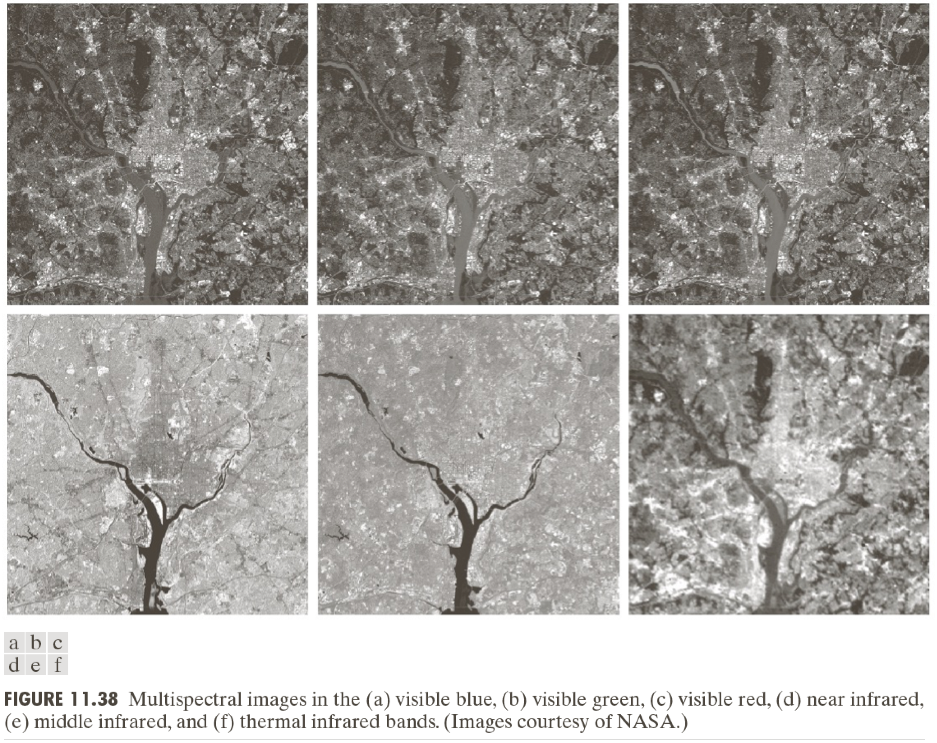
\includegraphics[width=10cm]{pca_1.png}
	\end{figure}
}

\frame
{
	\frametitle{Principal Components: Applications}
	\selectlanguage{english}
	\begin{figure}
		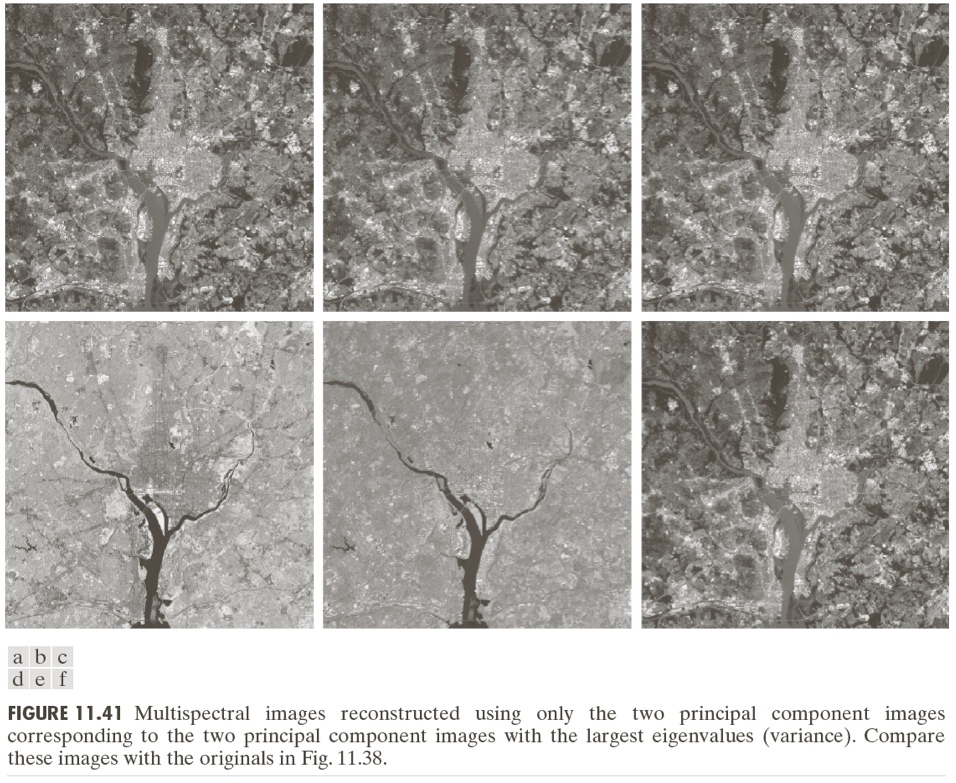
\includegraphics[width=10cm]{pca_2.png}
	\end{figure}
}


\frame
{
	\frametitle{Principal Components: Applications}
	\selectlanguage{english}
	\large	
	
	\begin{equation}
	\nonumber
	\begin{split}
	\text{\textbf{y}} 
	&= \text{\textbf{A}} (\text{\textbf{x}} - \text{\textbf{m}}_\text{\textbf{x}})
	\end{split}
	\end{equation}
	\begin{alertblock}{Properties of \textbf{y} }
		Transformed features \textbf{y} has the following advantages compared to \textbf{x}:
		
		\begin{enumerate}
			\item Invariant to translation and rotation 
			\begin{itemize}
				\item \textbf{y} has been shifted to the centroid by $\text{\textbf{m}}_\text{\textbf{x}}$
				\item \textbf{y} has been aligned with principal directions (eigenvectors)
			\end{itemize}
			\item Invariant to scaling can be achieved by dividing \textbf{y} for eigenvalues.
			
		\end{enumerate}
	\end{alertblock}
	
}

\frame
{
	\frametitle{Principal Components: Applications}
	\selectlanguage{english}
	\begin{figure}
		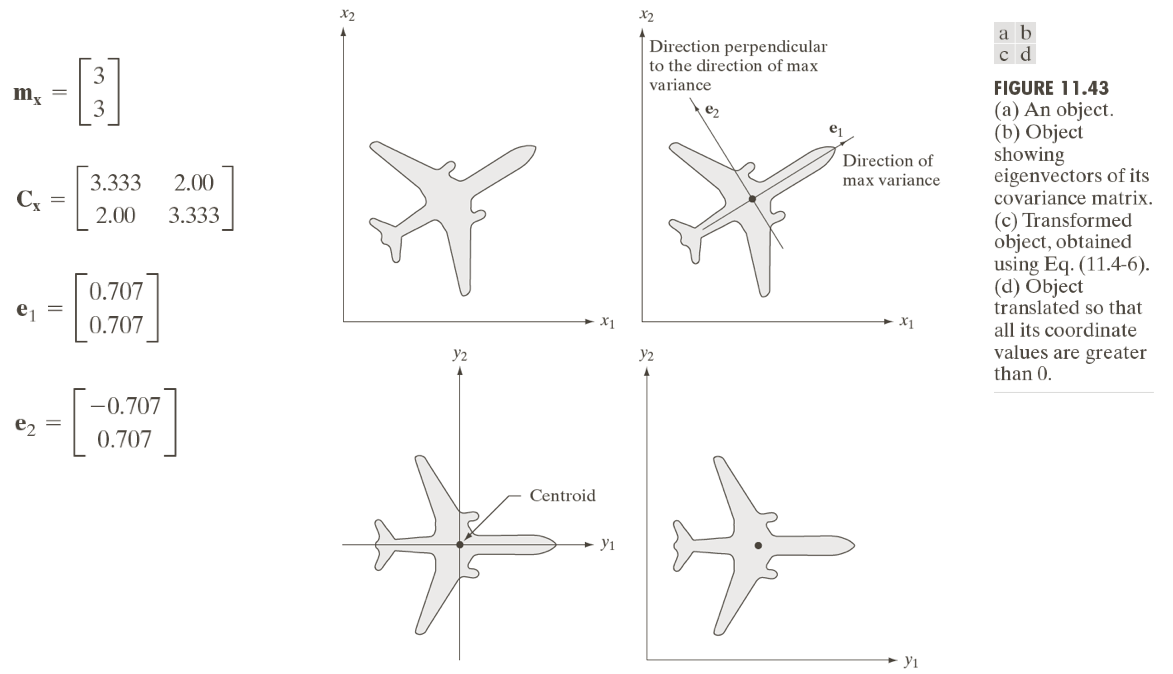
\includegraphics[width=10cm]{pca_3.png}
	\end{figure}
}


%%%%%%%%%%%%%%%%%%%%%%%%%%%%%%%%%%%%%%%%%%%%%%%

%%%%%%%%%%%%%%%%%%%%%%%%%%%%%%%%%%%%%%%%%%%%%%%

\end{document}